\chapter{Introduction}	\label{ch:introduction}
% What is DG and why use it?
High order discretization methods is a topic which has been gaining increasing attention in the last decades. An important exponent of them is the \gls{DG} method. The DG method was initially developed for solving hyperbolic conservation laws, and has recently gained increased attention for incompressible \gls{CFD} problems for structured and unstructured grids. Two main advantages stand out when compared with traditional methods such as the Finite Volume Method (FVM) or the Finite Difference Method (FDM): First, DG offers an arbitrary order of error convergence due to the local polynomial approximation of the solution field. A polynomial approximation of degree $p$ provides a numerical discretization error of the order  $\mathcal{O}(h^{p+1})$ for sufficiently smooth solutions, where $h$ is a characteristic grid length. In contrast, more traditional schemes, such as the FVM, are usually limited to $\mathcal{O}(h^N)$ accuracy, with $N \leq 2$ for unstructured grids. Even for structured grids $N$ is practically limited to low values due to the increasing stencil size for increasing $N$. 
Secondly, regardless of the desired order of accuracy, any given cell of the grid only requires information from its immediate neighbours, allowing an efficient parallelization with minimal communication overhead. Advantageously the DG method offers the locality of low-order schemes and the accuracy per \gls{dof} of spectral schemes, meaning that the same accuracy of a low-order scheme can be archived with less \gls{dof}. Other characteristic of the DG method is its ability to handle unresolved flows \parencite{henninkLowMachNumberFlow2022}, since by construction the weak form of the equations can be written as a local conservation law for each mesh element, bringing stability to the system.\\

%DG For combustion
High order methods are very attractive for complex reacting fluid dynamical systems, where usually a high numerical resolution is necessary. Particularly for combustion problems, where large amounts of heat are released in rather small zones within the flow, the high number of elements required to resolve the resulting steep gradients could result in prohibitive calculation times even for simple problems. In particular the study of so-called diffusion flames -- also known as non-premixed flames -- requires special consideration. In a diffusion flame, the reactants are initially spatially separated. For this kind of system, mixing plays a crucial role because reactants need to be brought together to the flame zone in order to maintain combustion. The use of a higher-order method, such as the DG method, can alleviate much of the need for high numerical resolution of combustion applications.\\

%% Diffusion flames and lowMach
Many practical applications of diffusion flames consider deflagration flames \parencite{poinsotTheoreticalNumericalCombustion2005} which are characterized by a small characteristic velocity compared to the speed of sound. The low-Mach approximation of the Navier--Stokes equations is often chosen for describing this kind of system. This approximation allows for the calculation of non-constant density flows while neglecting acoustic effects, thus dramatically reducing the required temporal resolution. This is crucial for the usability of explicit time marching algorithms, but also helpful for implicit schemes \parencite{mullerLowMachNumberAsymptoticsNavierStokes1998}.\\

%% Why the one step model
The need to accurately and efficiently represent the chemical reactions governing the combustion problem poses a major challenge. Generally speaking, to study the combustion process a detailed chemistry description is preferable. However, this is often impractical as it can be very intensive computationally speaking. Simplified kinetic models have been developed to overcome this difficulty, such as the one presented by \textcite{fernandez-tarrazoSimpleOnestepChemistry2006} for hydrocarbon combustion with air, where kinetic parameters are correlated to the equivalence ratio in order to better describe characteristic flame properties of premixed and non-premixed flames. By making use of a single chemical equation, it is possible to study complex combustion phenomena, substantially reducing the computational cost.  The model  offers a simple and versatile way to represent phenomena that would only be possible to predict using a more complex chemical model, for example the flame temperatures, near-extinction diffusion flames and reactant leakage.\\

%We choose this chemical model to obtain physically correct results for a wide range of applications, while avoiding the use of complex chemistry models. 

%% Method of resolution of the coupled solver 
The resolution of the discretized system of equations can be carried out using different strategies. One popular strategy is the SIMPLE-algorithm, originally developed by \parencite{patankarNumericalHeatTransfer1980} using a \gls{FDM}. Extention of the SIMPLE-algorithms for other discretization methods have been done, see \parencite{ferzigerComputationalMethodsFluid2002} for a \gls{FVM} and \parencite{haroutunianSegregatedFiniteElement1993} for a \gls{FEM}. An extention using the \gls{DG} has been done at the department of fluid dynamics at the TU-Darmstadt and is presented in the PhD thesis from \textcite{kleinHighorderDiscontinuousGalerkin2015}

%Conservative High-Order Finite Difference
%Schemes for Low-Mach Number Flows
%F. Nicoud 1
%owever, for the particular class of flow with
%low Mach number M and strong density variation, the classical compressible Navier-Stokes equations are not well suited for computation. The small time step limitation dictated by numerical stability requirements of explicit
%methods would require excessive computing times to solve practical flow
%problems. Indeed the sound waves move much faster than entropy or vorticity waves when M << 1. At the same time, in flows where the dominating
%mechanism is free, forced or mixed convection, the acoustical mode of energy
%carries only a small fraction of the energy present in the fluctuating part of
%the flow. These observations led several authors [1, 2, 3, 4] to propose a set
%of low-Mach number equations which do not contain acoustic waves but can
%still describe the entropy and vorticity modes as well as compressibility due
%to exothermicity of chemical reactions. A fractional-step method is used
%most often, the pressure field being obtained by solving a Poisson equation
%with the time derivative of the density field as part of the source term [3, 5].


%% Esto viene de la discusion de resultados: ya lo quite de ahi, asi que hay que ponerlo aca
%%% It was also observed that the calculation times were prohibitively high for some test cases. This point motivated the development of the solver presented in the present work, where the system is solved in a monolytic way and  and the Newton method globalized with a Dogleg-type method is used to solve the system.

% En la introduccion deberia dar una motivacion de porque esto es asi y porque se creó el solver fully coupled sin SIMPLE
%TODO \todo[inline]{what are exactly the advantages of the present solver? multigrid? Ortogonalization?} 

The \gls{BoSSS} code 


\section{Motivation and objectives of this work}

In one of the early stages of the implementation of the low-Mach solver the SIMPLE algorithm was adopted for the solution of the velocity-pressure coupling of the governing flow equations. Although this strategy was able to solve various variable density test-configurations, it was observed that the computation times were under certain conditions very high. The solution method includes the use of fixed point iterations, which often require the use of under-relaxation factors, which if not well chosen can dramatically increase the computation time. This was the main motivation for the development of the present solver, which from this point on will be called \gls{XNSEC}. The term \textit{extended} refers to the framework on which the solver is built, which focuses on applications for multi-phase flows using a sharp interface approach using a level-set method. 

The strategy proposed in the present work proposes a fully coupled solution of the system of equations. The non-linear system is solved using a Newton algorithm, and the associated linear problems are solved with a dedicated software (PARDISO). As an example that motivates the development and use of the \cref{fig:RuntimeComparisonk2} strategy, a comparison of the computation times for the same case using a fully coupled approach (XNSEC) and the SIMPLE algorithm is shown 

\begin{figure}[h]	
	\centering
	\inputtikz{RuntimecomparisonWithSimple_k2}
	\caption{Runtime comparison of the DG-SIMPLE solver and the XNSEC solver on a typical simulation.}
	\label{fig:RuntimeComparisonk2}
\end{figure}
Although both algorithms allow the simulation of low-Mach number flows, clearly the SIMPLE algorithm requires much more time. This is by no means an indication that the resolution using a fully implicit scheme is in general superior to a strategy such as the SIMPLE algorithm in the context of DG-methods, and possibly further optimization of the segregated algorithms could lead to an improvement in computation times.


In the present work, a low-Mach pressure-based solver for the simulation of temperature dependent non-reactive and reactive flows using the Discontinuous Galerkin method is presented. To the best of the authors knowledge, this is the first time that a pressure-based solver is used together with the DG method for solving the low-Mach equations using a Newton method in a fully coupled manner. We focus in this study on two-dimensional configurations, but the ideas presented could be extended to three-dimensional systems. The one-step combustion model presented by Fernandez-Tarrazo et al. \textcite{fernandez-tarrazoSimpleOnestepChemistry2006} is used for describing the chemical reactions. In the present work we consider only methane combustion, but the one-step model could be used for other hydrocarbons as well. The discrete system of equations is solved by a globalized Newton method, by means of the Dogleg approach. In addition to the Newton-Dogleg method, a homotopy strategy is presented, which was found to be useful for obtaining solutions of steady state calculations of highly nonlinear problems. In order to find appropriate initial values for Newton's method in combustion applications, the concept of flame sheet estimates (i.e. the solution for infinitely fast chemistry) is used. Several benchmark cases are presented that allow us to validate our implementation. First we solve the differentially heated cavity problem, with which we intend to validate our implementation of the low-Mach solver for non-constant density flows using the fully coupled solver. Later two flame configurations are calculated, namely the counter-diffusion flame and the chambered diffusion flame. \parencite{matalonDiffusionFlamesChamber1980}

\section{Outline of the thesis}

The thesis is structured as follows: In \cref{ch:gov_eqs} the low-Mach number Navier-Stokes set of equations is presented. The chapter begins by presenting the governing equations in a general way, and concisely shows the main elements for the derivation of the low Mach equations, emphasizing the assumptions made to arrive at them, as well as the models for the different parameters involved in the simulation. In addition, the chemical model chosen for the combustion simulation is presented. Later in \cref{sec:FlameSheet} the concept of the flame-sheet and the Burke-Schumann limit, which are used within the solution algorithm for combustion cases, is shown. 

In \cref{ch:NumericalMethods} the numerical method used in this work is presented. First, a brief introduction to the DG-method is given using a simple transport equation, which allows demonstrating the procedure used for the spatial and temporal discretization of the governing equations. Then in \cref{ssec:nonLinearforms} a description of each of the discretized terms of the governing equations is shown, with special emphasis on the numerical fluxes involved.

The methods for solving the system of discretized equations are presented in \cref{ch:CompMethodology}. The chapter starts with a description of the solver structure, showing the basic building blocks of it. In \cref{sec:SolNonLinProblem} the globalized Newton method used to solve the fully coupled non-linear system is shown. Emphasis is placed on the basic functioning of the method, as well as on certain computational aspects that allow for a higher efficiency. Additionally, in \cref{sec:ConvSupportStrat} additional strategies are presented that improve the convergence properties of the method for cases where the newton algorithm is not able to obtain solutions, such as the use of the flame-sheet estimates for combustion simulations and homotopy methods for highly non-linear problems.

In \cref{ch:results} a comprehensive testing of the solver using a variety of test cases is presented. These test cases are compared with benchmark results, but are also used for highlighting the algorithms introduced in this work. The test cases presented are subdivided in three sections, in increasing level of complexity. First, in \cref{sec:SingleCompIsotCase} the solver is used to calculate typical incompressible benchmark cases, such as lid-driven cavity flow or a backward-facing step, and the results are compared with benchmark solutions. Then in \cref{sec:SinCompNonIsothermCase} the tests are extended to low-Mach number flows, and several typical configurations are calculated for such systems, in particular problems where the temperature has an influence on the flow field, such as the heated square cavity configuration (\cref{ss:DHC}), and the Rayleigh-Bénard Convection problem (\cref{ssec:RayBer}).
Finally in \cref{sec:MultCompNonIsothermCase} the fully coupled system of equations for reactive low-Mach flows is used for calculating some typical diffusion flame configurations. In \cref{ssec:coflowFlame} a coflow flame configuration is simulated. Later in \cref{ss:CDF} a planar counterflow flame configuration is calculated, and the results are compared with simulations of a one-dimensional configuration. 

Finally, a conclusion of the work is done in \cref{ch:conclusion}.


Many parts of the present thesis are based on \textcite{gutierrez-jorqueraFullyCoupledHigh2022}, which has been published by the author of this work.


\section{The BoSSS code}
The presented solver is embedded in the \gls{BoSSS} code, which is under active development at the chair of fluid dynamics of the Technical University of Darmstadt, and is available under \href{https://github.com/FDYdarmstadt/BoSSS}{https://github.com/FDYdarmstadt/BoSSS}.

BoSSS is a general framework for the discretization of conservation laws using the DG method and uses a modal DG approach with orthonormal Legendre polynomials as basis functions. The BoSSS code features a variety of applications in the context of computational fluid dynamics, such as a solver for multiphase flows with a sharp interface approach \parencite{kummerExtendedDiscontinuousGalerkin2017}, an incompressible Immersed Boundary Method solver for particle laden flows \parencite{krauseIncompressibleImmersedBoundary2017}, a solver for viscoelastic fluid flows\parencite{kikkerFullyCoupledHighorder}, and a solver for compressible flows \parencite{geisenhoferDiscontinuousGalerkinImmersed2019}, among others.

The structure of the BoSSS framework is shown in a schematic way in \cref{Fig:BoSSS}. BoSSS allows the end user to develop sophisticated solvers at a very low coding effort. The implementation makes extensive use of several \gls{MPI}-parallel, performance-optimized operations, among which the evaluation of the DG operator can be highlighted, as well as a solution using parallelized algorithms for the resolution of linear systems arising from the discretization. In addition, the user has at his disposal a large number of tools that optimize the workflow, such as the use of Jupyter-notebooks, as well as various post-processing tools.
\begin{figure}
	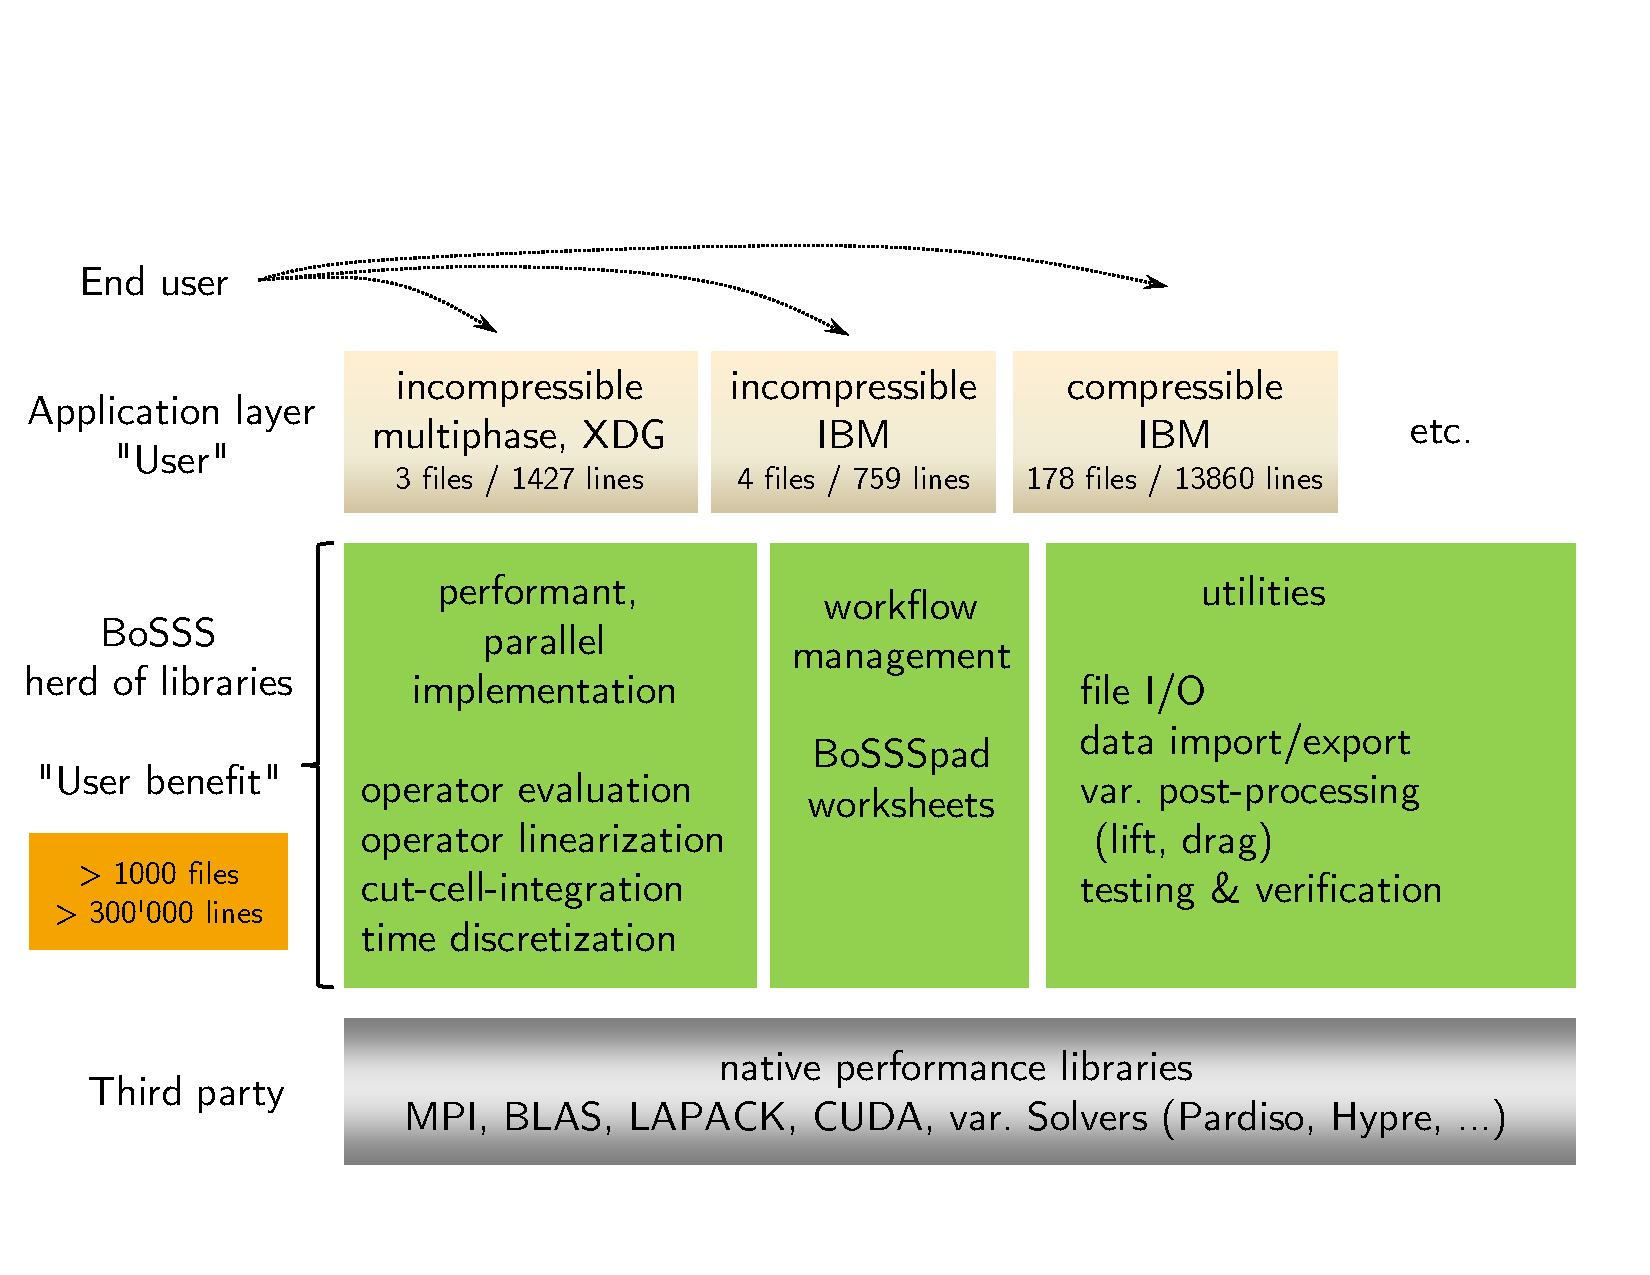
\includegraphics[width=\textwidth]{BoSSS-philosophy-1.pdf}
	\caption[Schematic representation of the structure of the BoSSS solver.]{Schematic representation of the structure of the BoSSS solver. Extracted from the BoSSS handbook \parencite{kummer2020}.}
	\label{Fig:BoSSS}
\end{figure}

